\documentclass[a4paper, 10pt]{article}

% import packages
\usepackage[margin=0.2cm]{geometry}
\usepackage{pdflscape}
\usepackage{array}
\usepackage{makecell}
\usepackage{xcolor}
\usepackage{colortbl}
\usepackage{longtable}
\usepackage{titlesec}
\usepackage{float}
\usepackage{needspace}
\usepackage{graphicx}
\usepackage{hyperref}
\usepackage{setspace}
\usepackage{fancyhdr}
\usepackage{enumitem}
\usepackage{multicol}
\usepackage{amsmath}
\usepackage{graphicx}
\usepackage[table]{xcolor}
\usepackage{booktabs}   % for \toprule, \midrule, \bottomrule
\usepackage{adjustbox}  % for \begin{adjustbox}{max width=\textwidth}
\usepackage{etoolbox}
\usepackage{tikz}
\usepackage{caption}
\usetikzlibrary{arrows.meta, positioning, shapes.geometric,fit,calc}

\AtBeginEnvironment{tabular}{\tiny}
\definecolor{cDark}{HTML}{203F4A}
\definecolor{cTeal}{HTML}{1D8F7E}
\definecolor{cGold}{HTML}{E9C06A}
\definecolor{cOrange}{HTML}{F29B5C}
\definecolor{cRed}{HTML}{E85D47}

\renewcommand{\familydefault}{\sfdefault}

\newlength\tindent
\setlength{\tindent}{\parindent}
\setlength{\parindent}{0pt}
\renewcommand{\indent}{\hspace*{\tindent}}

% global list spacing (affects all levels)
\setlist{noitemsep, topsep=0pt, parsep=0pt, partopsep=0pt}


% now explicitly override indentation for each level you care about:
\setlist[itemize,1]{leftmargin=1.2em,label=\raisebox{0.5ex}{\scalebox{0.6}{$\bullet$}}}
\setlist[itemize,2]{leftmargin=1.4em}
\setlist[itemize,3]{leftmargin=0.5em,label=\raisebox{0.5ex}{\scalebox{0.6}{$\bullet$}}}


\setlist[enumerate,1]{leftmargin=1.2em}
\setlist[enumerate,2]{leftmargin=1.4em}
\setlist[enumerate,3]{leftmargin=0.5em}

\setlength{\columnseprule}{0.1pt}
% ------------------------------------------------------


% Configure makecell package
\renewcommand{\theadalign}{bc}
\renewcommand{\theadgape}{\Gape[4pt]}
\renewcommand{\cellgape}{\Gape[4pt]}
\renewcommand{\cellalign}{lt}

% global line spacing
\renewcommand{\baselinestretch}{1.2}

% colour definitions
\definecolor{lightergray}{gray}{0.90}

\providecommand{\tightlist}{%
\setlength{\itemsep}{0pt}
\setlength{\parskip}{0pt}}

\begin{document}
  \begin{landscape}

\begin{multicols}{5}

\tiny

\begin{itemize}
    \item \texttt{?} \(\rightarrow\) 0-1
    \item \texttt{*} \(\rightarrow\)  0-n
    \item \texttt{+} \(\rightarrow\) 1-n
    \item \texttt{*?} \(\rightarrow\) 0-n (lazy)
\end{itemize}



\vspace{0.4em}
\hrule
\vspace{0.7em}

{\footnotesize{General}}

\begin{itemize}
    \item Token: input of NLP
    \item Corpus: collection of words and phrases, can be mixed source
    \item Vocabulary: set of words known to an NLP system or dataset
    \item Out of Vocabulary: wort nicht im vocabulary can be because of spelling mistakes, etc.
    \item Zipf's Law
    \begin{itemize}
    \item word by frequency rank
    \item frequency of word is about inverse proportianal to its rank
    \item "power low"
\end{itemize}
\end{itemize}

\vspace{0.4em}
\hrule
\vspace{0.7em}

{\footnotesize{Cleaning \& Preprocessing}}

\begin{itemize}
    \item Zu seltenes Wort \(\rightarrow\) weg, unklar wie umgehen
    \item Zu häufiges wort \(\rightarrow\) weg, nicht aussagekräftig
    \item remove special characters, links, html tags
    \item normalise whitespaces
    \item fix encoding
    \item Stop Words: removal common words, custom
    \item reduce variety of words
    \begin{itemize}
        \item Stemming: word stem (remove suffix)
        \item lemmatisation
    \end{itemize}
    \item n-grams: \# wörter pro token 
    \item Tokenisation: separate text strings into sentences and words
    \item Spelling Error Correction
    \begin{itemize}
        \item incorrect is out of vocab
        \item Deterministic approach, eg. levenstein Distance (1 means 1 change)
        \item you are allowed to make x edits. If you can reach a word in vocab you are allowed to do that
    \end{itemize}
    \item Part of Speech Tagging: classify word (adjective, etc.)
    \item Named Entity Recognition
\end{itemize}

\vspace{0.7em}

{\footnotesize{NLP Pipeline}}

\begin{itemize}
    \item Text Data (Corpus)
    \item Text Pre-processing (stopwords, etc.)
    \item Vectorisation (to numbers) \(\rightarrow\) bag of words
    \item ML Model with nummerical data
\end{itemize}


\vspace{0.4em}
\hrule
\vspace{0.7em}

{\footnotesize{Evaluation}}

\begin{itemize}
    \item measures qualities of an algorith / system
    \item proper criteria is essential
    \item metrics and evaluation data is required
    \item Automatic
    \begin{itemize}
        \item oftmals
        \item comparing output with gold standard
        \item gold standard data is costly
    \end{itemize}
    \item Manual
    \begin{itemize}
        \item quick and dirty by humans based on criteria
        \item form many NLP problems creating gold standard is impossible or expensive
    \end{itemize}
    \item Intrinsic: isolated on the NLP system itself
    \item Extrinstic: NLP system as part of a larger complex system
    \item Inter-Annotator Agreement
    \begin{itemize}
        \item How good are my labels)
        \item consistency measurement: how consistent do diff. annotators do it?
        \item reliability indicator: high suggests reliable / constant interpretation
        \item done through various methods
        \item important for tasks with subjective judgements
    \end{itemize}
    \item Accuracy: percentage of correctly predicted instances
    \item Precision: \(\dfrac{TP}{TP + FN}\) what part of positive is actually correct?
    \item Recall: \(\dfrac{TP}{TP + FN}\) what proportion of actual positives was correctly identified
    \item F1-Score (weighted harmonic mean): \\ \(F_1 = 2 \cdot \dfrac{Precision \cdot Recall}{Precision + Recall}\)
    \item Precision at K
    \begin{itemize}
        \item some cases precision impossible (search results on internet)
        \item take precision at top 10 (P10) what proportion of top 10 documents are relevant
        \item disadvantage does not take order in consideration
    \end{itemize}
    \item verify label through confusion matrix
\end{itemize}
\vspace{0.7em}

{\footnotesize{Baseline}}
\begin{itemize}
    \item important
    \item starting point: metric of a simple system to evaluate a more complex system
    \item Benchmarking: is new genuinelly better than simple?
    \item simplicity \& clarity: should be easy to implement and reproduce
    \item realistic expectations: context for improvement help set realistic goals
    \item progress measurement is crucial
\end{itemize}

\vspace{0.4em}
\hrule
\vspace{0.7em}

{\footnotesize{Neural Networks in NLP}}

\begin{itemize}
    \item NN = matrix multiplications + non-linearities
    \item text \(\rightarrow\) numbers \(\rightarrow\) tensors  \(\rightarrow\) NN  \(\rightarrow\) predictions
\end{itemize}

\vspace{0.7em}

{\footnotesize{Simple Neural Classifier}}

\begin{itemize}
    \item Classify text documents into categories (like spam-filter)
    \item Input: Text document, output: pre-defined categories
    \item Training
    \begin{enumerate}
        \item Initialisation: random weights
        \item Forward Pass: input \(\rightarrow\) NN \(\rightarrow\) prediction with softmax
        \item Loss: How wrong?
        \item Backward Pass: compute gradients
        \item Update weights: improve NN
        \item Repeat x times
    \end{enumerate}
\end{itemize}


\vspace{0.4em}
\hrule
\vspace{0.7em}

{\footnotesize{Embeddings}}

\begin{itemize}
    \item example word2vec
    \item Problem Bag of Words: see other
    \item Embeddings: dense low dimensional, learned representations
    \item it is a normal hidden layer if input is sparse vector better to first reduce it
    \item Properties
    \begin{itemize}
        \item Dense: all values in vector are meaningful
        \item Low Dimensional
        \item Learned: trained as layer if in NN
        \item Semantic: similar words have similar vectors
        \item no activation function
    \end{itemize}
    \item Embedding Matrix: 1 row per word, lookup for word
    \item Use-cases
    \begin{itemize}
        \item Text generation, improvement of text
        \item chatbot to get explanations
        \item text to SQL
        \item software
    \end{itemize}
\end{itemize}


\vspace{0.4em}
\hrule
\vspace{0.7em}

{\footnotesize Attention (Transformer Core)}

\begin{itemize}
    \item \textbf{which parts of a sequence matter most} for each token
    \item Instead of reading strictly left-to-right, attention lets each token measure its \textbf{relevance to other tokens} and build a \textbf{context-aware representation}.
    \item models \textbf{token-to-token relevance}
    \item strengthens \textbf{important context}
    \item creates each output token as a \textbf{weighted combination of previous tokens}
\end{itemize}

\textbf{Example:}  
Sentence: \textit{``The animal didn't cross the street because it was tired.''}  
The token \textbf{``it''} should attend strongly to \textbf{``animal''} (not \textbf{street}), because that resolves the meaning.

\vspace{0.4em}

{\footnotesize Self-Attention}

In \textbf{self-attention}, each token can “look at” \textbf{all other tokens} (including itself). This allows the model to capture:
\begin{itemize}
    \item \textbf{local dependencies} (nearby words)
    \item \textbf{long-range dependencies} (far relationships)
    \item richer \textbf{contextual embeddings}
\end{itemize}

Self-attention produces \textbf{new embeddings} that are more informative than the input embeddings.

\textbf{Example (long-range dependency):}  
\textit{``The book that the professor recommended was expensive.''}  
The token \textbf{``was''} must attend to \textbf{``book''} (the true subject), even though they are far apart.

\vspace{0.4em}
{\footnotesize Query / Key / Value (Q / K / V)}

Each token is projected (via learned weight matrices) into three vectors:
\begin{itemize}
    \item \textbf{Query (Q):} what the current token is looking for
    \item \textbf{Key (K):} what each token offers as “matchable information”
    \item \textbf{Value (V):} the information each token contributes if selected
\end{itemize}

\textbf{Quick intuition:}  
\textbf{Query} = “What do I need?”  
\textbf{Key} = “What do I contain?”  
\textbf{Value} = “What information do I pass on if chosen?”

\textbf{Example:}  
Sentence: \textit{``Alice gave Bob her book.''}  
For token \textbf{``her''}:  
\begin{itemize}
    \item Query asks: “Whose?”  
    \item Keys from \textbf{Alice}, \textbf{Bob} compete as possible owners  
    \item Attention weight becomes larger for \textbf{Alice}, so \textbf{``her''} mixes more of Alice’s value vector.
\end{itemize}

{\scriptsize How it works:}
\begin{enumerate}[leftmargin=1.8em]
    \item Compare current token’s query with all keys:
    \(Q \cdot K^\top\)
    \item Scale scores by $\sqrt{d_k}$ to keep values stable
    \item Apply a \textbf{mask} (for causal models) to block future tokens
    \item Apply \textbf{softmax} to get attention weights
    \item Compute weighted sum of values:
    \( \text{weights} \times V \rightarrow \text{context output} \)
\end{enumerate}

\textbf{Mask example (causal language model):}  
In \textit{``I eat pizza''}, when predicting \textbf{``eat''}, the model may attend to \textbf{``I''} but cannot attend to \textbf{``pizza''}, because it lies in the future.

\textbf{Key insight:}  
Each token becomes a weighted mixture of \textit{all} value vectors, where weights depend on how well the query matches the keys.

\vspace{0.4em}
\hrule
\vspace{0.7em}

{\footnotesize Multi-Head Attention (MHA)}

Transformers run \textbf{multiple self-attention heads in parallel}. Each head has its own learned projection matrices:
\(Q = XW_Q,\quad K = XW_K,\quad V = XW_V\)

This allows each head to learn a different alignment rule over the same input.

\vspace{0.3em}
\textbf{Why multiple heads?}

A single attention head produces only \textbf{one attention pattern} --- a limited view. With multiple heads, the model can attend to different kinds of relationships \textbf{simultaneously}.

Heads often specialize in:
\begin{itemize}
    \item syntax (subject--verb, nearby dependencies)
    \item semantics (topic/meaning connections)
    \item coreference (pronouns $\rightarrow$ entities)
    \item local vs long-range patterns (short vs far dependencies)
\end{itemize}

\vspace{0.3em}
\textbf{How it works (high level)}

Each head computes scaled dot-product attention:
\(
\text{Attention}(Q,K,V)=\text{softmax}\left(\frac{QK^\top}{\sqrt{d_k}}\right)V
\)

Outputs from all heads are:
\begin{itemize}
    \item \textbf{concatenated} (wider feature space)
    \item passed through a \textbf{final linear projection} $W_O$ to mix information back into $d_{\text{model}}$
\end{itemize}

\vspace{0.3em}
\textbf{Example:}  
Sentence: \textit{``The scientist who won the award wrote a paper.''}

\begin{itemize}
    \item One head may link \textbf{``scientist''} $\rightarrow$ \textbf{``wrote''} (grammatical dependency)
    \item Another head may focus inside \textbf{``who won the award''} (relative clause)
    \item Another head may connect \textbf{``won''} $\leftrightarrow$ \textbf{``award''} (semantic association)
\end{itemize}

\textbf{Key idea:}  
Each head is a different perspective on the same sentence --- combining them produces richer token representations.

\vspace{0.4em}
\hrule
\vspace{0.7em}



{\footnotesize Transformer Language Model (Decoder-Style)}

A decoder-style transformer is designed for \textbf{next-token prediction}. It uses self-attention with a causal mask so that each token can only attend to earlier positions.

\begin{itemize}
    \item \textbf{Masked self-attention:} prevents future information leakage  
    (token at position $t$ can only attend to positions $\leq t$)
    \item \textbf{Positional encoding:} attention has no built-in notion of order, so positional information is injected into embeddings (sinusoidal or learned)
    \item \textbf{Feed-forward network (FFN):} applied independently to each token, expanding and compressing dimensions:
    \(
    d_{\text{model}} \rightarrow d_{\text{ff}} \rightarrow d_{\text{model}}
    \)
    adds nonlinearity beyond attention
    \item \textbf{Residual connections:} input is added back after each sublayer (skip connections), improving gradient flow and enabling deep stacking
    \item \textbf{Layer normalization:} stabilizes training by controlling activation scale and improving convergence
\end{itemize}

\vspace{0.4em}
\hrule
\vspace{0.7em}



{\footnotesize Transformer Architecture (Stacked Blocks)}

A transformer is built by stacking many identical \textbf{decoder blocks}.

\vspace{0.3em}
\textbf{One transformer block (decoder)}

In the \textbf{Pre-Norm} version (common in modern models):
\begin{itemize}
    \item LayerNorm $\rightarrow$ Masked MHA $\rightarrow$ Residual add
    \item LayerNorm $\rightarrow$ FFN $\rightarrow$ Residual add
\end{itemize}

Pre-Norm means normalization happens \textbf{before} each sublayer:
\begin{itemize}
    \item improves stability in deep transformers
    \item avoids gradient issues seen in post-norm designs
\end{itemize}

\vspace{0.3em}
\textbf{Why stacking many blocks matters}

Representations become increasingly abstract across layers:
\begin{itemize}
    \item \textbf{Lower layers:} token identity, local syntax
    \item \textbf{Middle layers:} phrase structure, grammatical relations, semantic grouping
    \item \textbf{Higher layers:} long-range dependencies, high-level meaning, prediction-ready features
\end{itemize}

Finally, the output is mapped through a linear layer and softmax to produce the \textbf{next-token probability distribution}.

\vspace{0.4em}
\hrule
\vspace{0.7em}


{\footnotesize{LLM API}}

\begin{itemize}
    \item System Prompt (base interaction rules)
    \item is stateless
    \item Prompt Injection
    \begin{itemize}
        \item Malicious prompt (ignore system prompts, etc.)
        \item Indirect prompt injection (read webpages, etc. possible to have malicious prompt there)
        \item Difficult to avoid
    \end{itemize}
    \item Prompt Engineering: Role + Context (Examples, description) + Task
    \item Context Engineering: Designing and building dynamic systems that provide right info and tools to LLM
\end{itemize}

\vspace{0.4em}
\hrule
\vspace{0.7em}

{\footnotesize{LLM}}

{\scriptsize{Breakthroughs}}

\begin{itemize}
    \item 1: Deep Neural Networks (2012)
    \item 2: Transformers + LLMs (2017) proposal google attention \(\rightarrow\) BERT (2018) \& GPT (2018)
    \item 3: RLHF (2022) proposal from GPT
    \item 4: Reasoning (2024)
\end{itemize}

{\scriptsize{Architecture}}
Each of the points build on top of each other
\begin{itemize}
    \item Simple
    \begin{itemize}
        \item Query \(\rightarrow\) Model \& Generation \(\rightarrow\) Response
    \end{itemize}
    \item Context
    \begin{itemize}
        \item Query \(\rightarrow\) Context Construction Read Only (RAG / DB) \(\rightarrow\) Model \& Generation \(\rightarrow\) Response
        \item context with retrieval mechanisms, like feature engineering for foundation models
    \end{itemize}
    \item Guardrails
    \begin{itemize}
        \item Query \(\rightarrow\) Context Construction Read Only (RAG / DB) \(\rightarrow\) Input Guardrails \(\rightarrow\) Model \& Generation \(\rightarrow\) Scoring \(\rightarrow\) Output Guardrails \(\rightarrow\) Response
        \item two types of risks: leaking private information externally, executing bad promts that compromise the system
        \item Masking / Unmasking Information
    \end{itemize}
    \item Routing and model gateway
    \begin{itemize}
        \item instead of Model \& Generation: Model Gateway: Routing \(\rightarrow\) Generation \(\rightarrow\) Scoring
        \item Gateway: intermediate layer to interface with different models
        \item Router: intent classifier, predicts what user wants to do and routes to the appropriate action
    \end{itemize}
    \item Agent
    \begin{itemize}
        \item Layer to orchestrate sequence of actions and tools
    \end{itemize}
\end{itemize}


\vspace{0.4em}
\hrule
\vspace{0.7em}


{\footnotesize{Chatbots}}

\begin{itemize}
    \item {\textbf{Definition:}} LLM that is finetuned to follow instructions
    \item {\textbf{Chain-of-Thought:}} Input is Example question and answer, then also provide real question
    \item {\textbf{Reasoning LLMs:}} Question, "thinks" several times before providing answer
    \item {\textbf{Challenges:}} Legal, Privacy, Service is down, price, societal implications
\end{itemize}


Reinforcement Learning from human feedback (RLHF)
\begin{itemize}
    \item Supervised fine-tuning
    \begin{itemize}
        \item starts with pre-trained LLM
        \item supervised fine-tuning on high quality human demonstrations establishing baseline
    \end{itemize}
    \item Reward model training
    \begin{itemize}
        \item Human rank / rate multiple output for same promt
        \item Preference data trains separate reward model (other transformer), learns to predict human preference
    \end{itemize}
    \item Policy Optimisation
    \begin{itemize}
        \item LLM fine-tuned with reinforcement learning, for maximal learned reward score while maintaining constraints from original model
    \end{itemize}
    \item Evaluate on unseen tasks
\end{itemize}


\vspace{0.4em}
\hrule
\vspace{0.7em}

{\footnotesize{RAG}} Retrieval-Augmented Generation

\begin{itemize}
    \item Context information is retrieved
    \item Benefits
    \begin{itemize}
        \item Reduces hallucinations
        \item Low cost, no training / finetuning
        \item Explainability, can provide citations
    \end{itemize}
\end{itemize}



\vspace{0.4em}
\hrule
\vspace{0.7em}

{\footnotesize{Agent}}

\begin{itemize}
    \item Issue with LLM
    \begin{itemize}
        \item only computes probability of next token
        \item limited computability: bad at logic for example math
        \item no inherent memory: stateless no knowledge of previous
    \end{itemize}
    \item Agency: ability to steer its own workflow
    \item Independently accomplish tasks
    \item When to use agents?
    \begin{itemize}
        \item Complex Decision making: context sensitive, exceptions, etc.
        \item Difficult to maintain rules: systems with complicated rule set
        \item Heavy reliance on unstructured data: interpreting natural languages
    \end{itemize}
    \item Here too, find simplest answer, may not be an agent.
    \item Definition / Components
    \begin{itemize}
        \item Environments: world agent interacts with
        \item Sensors: used to observe environment
        \item Actuators: tools to interact with the environment
        \item Effectors: "brain", rules deciding how to go from observation to actions
    \end{itemize}
    \item Agent components
    \begin{itemize}
        \item Planning: Chain-of-Thoughts, Reflection, subgoal decomposition
        \item Tools: Search, API, function calling
        \item Memory: short / long-term, retrieval
        \item Autonomous Steps: plan \(\rightarrow\) Action (and back again)
    \end{itemize}
    \item Model Context Protocol (MCP)
    \begin{itemize}
        \item Standardised API services for services
        \item Host (LLM app) / Client (1:1 connection to server) / Server (provides context)
        \item For example, i need to do x, what can I use to do that?
    \end{itemize}
    \item Guardrails
    \begin{itemize}
        \item Layered Defense mechanism
        \item relevance classifiers: flags off-topic queries
        \item Safety classifier: detects unsafe input
        \item PII filter: prevents exposure personal info
        \item Moderation: flags harmful content
        \item Tool safeguards
    \end{itemize}
\end{itemize}

\vspace{0.4em}
\hrule
\vspace{0.7em}


3 Representations of text

{\scriptsize{Binary Bag-of-Words}}
\begin{itemize}
  \item Representation: High-dim vector over vocab; count of word appearance, else 0. Ignores order/frequency. No semantics
  \item When useful:
    \begin{itemize}
      \item TF-IDF, Simple classification/retrieval (e.g., spam, topic flags).
      \item Large-scale, fast, interpretable baselines (low compute, low semantics).
    \item Limitation: No Semantics, sparse mostly 0, no magnitude only presence or not, not how important
    \end{itemize}
\end{itemize}

{\scriptsize{Dense (non-contextual) embeddings}}
\begin{itemize}
  \item Representation: Low-dim continuous vectors for words/sentences (e.g., Word2Vec, GloVe); similar words $\rightarrow$ nearby vectors.
  \item When useful:
    \begin{itemize}
      \item Semantic similarity: clustering, nearest-neighbor search, retrieval.
      \item Fixed features when data/compute are limited (more compact than BoW).
    \end{itemize}
\end{itemize}

{\scriptsize{Contextualized transformer embeddings}}
\begin{itemize}
  \item Representation: Token vectors depend on full context via self-attention; same word $\rightarrow$ different vectors in different sentences. Sentence models can pool to one vector.
  \item When useful:
    \begin{itemize}
      \item Context-sensitive tasks: QA, NLI, nuanced sentiment, generation.
      \item Transfer learning: pretrained transformer embeddings + fine-tuning for best performance.
    \end{itemize}
\end{itemize}


\vspace{0.4em}
\hrule
\vspace{0.7em}

{\footnotesize{Recurrent Neural Networks (RNN)}}

\begin{itemize}
    \item problem with bag of words: no word order, no context
    \item RNN is sequential processing with memory
    \item Idea
    \begin{itemize}
        \item gets current embedding + previous hidden state (memory from previous input)
        \item creates new hidden state
        \item Hidden State = memory
        \item Final hidden state is output
    \end{itemize}
\end{itemize}

\vspace{0.4em}
{\scriptsize{Classification}}

\begin{itemize}
    \item Embeddings \(\rightarrow\) RNN \(\rightarrow\) final hidden state \(\rightarrow\) Classifier
    \item processes entire sequence
    \item final hidden state contains all context
    \item classify based on accumulated info
\end{itemize}


\vspace{0.4em}
{\scriptsize{Generation}}
\begin{itemize}
    \item From input more text
    \item LLM: probability distribution over sequences, for each position it predicts the probability of that word
    \item Autoregressive Generation: use your own output as inputs
    \item RNN for Lang Model: at each step predict next based on current hidden state
    \item Sampling Strategy
    \begin{itemize}
        \item Greedy: pick most likely word
        \item Random: pick any from probability distribution
        \item Temperature: controll randomness
        \item Low Temp: conservative / High Temp: creative, chaotic
    \end{itemize}
\end{itemize}

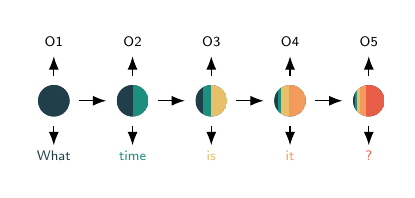
\begin{tikzpicture}[
    >=Latex,
    arrow/.style={-Latex, shorten >=1pt, shorten <=0.5pt},
    updown/.style={-Latex, shorten >=1pt, shorten <=0.5pt},
    lab/.style={font=\tiny},
    word/.style={font=\tiny},
]

% ---------- Helper macro: circle with vertical bands ----------
\newcommand{\tokencircle}[4]{%
  \begin{scope}
    \coordinate (C) at (#1,#2);
    \clip (C) circle (#3);
    \fill[cDark] (C) circle (#3);
    \foreach \xs/\xe/\col in {#4}{
      \fill[\col] ($(C)+(\xs*#3,-#3)$) rectangle ($(C)+(\xe*#3,#3)$);
    }
  \end{scope}
}

% ---------- Geometry (smaller + tighter) ----------
\def\r{0.2}      % smaller radius
\def\dx{1.00}     % tighter horizontal spacing
\def\y{0}

% ---------- Circles ----------
\tokencircle{0*\dx}{\y}{\r}{-1/1/cDark}

\tokencircle{1*\dx}{\y}{\r}{-1/0/cDark,0/1/cTeal}

\tokencircle{2*\dx}{\y}{\r}{-1/-0.55/cDark,-0.55/0/cTeal,0/1/cGold}

\tokencircle{3*\dx}{\y}{\r}{-1/-0.75/cDark,-0.75/-0.55/cTeal,-0.55/-0.05/cGold,-0.05/1/cOrange}

\tokencircle{4*\dx}{\y}{\r}{-1/-0.86/cDark,-0.86/-0.74/cTeal,-0.74/-0.54/cGold,-0.54/-0.18/cOrange,-0.18/1/cRed}

% ---------- Horizontal arrows ----------
\foreach \i in {0,1,2,3}{
  \draw[arrow] (\i*\dx+\r+0.1,\y) -- (\i*\dx+\dx-\r-0.1,\y);
}

% ---------- Vertical arrows + labels ----------
\foreach \i/\labtext in {0/O1,1/O2,2/O3,3/O4,4/O5}{
  \draw[updown] (\i*\dx,\y+\r+0.10) -- (\i*\dx,\y+\r+0.4);
  \draw[updown] (\i*\dx,\y-\r-0.10) -- (\i*\dx,\y-\r-0.4);
\node[lab] at (\i*\dx,\y+\r+0.55) {\labtext};
}

% ---------- Words under circles ----------
\node[word, text=cDark]   at (0*\dx,\y-\r-0.5) {What};
\node[word, text=cTeal]   at (1*\dx,\y-\r-0.5) {time};
\node[word, text=cGold]   at (2*\dx,\y-\r-0.5) {is};
\node[word, text=cOrange] at (3*\dx,\y-\r-0.5) {it};
\node[word, text=cRed]    at (4*\dx,\y-\r-0.5) {?};

\end{tikzpicture}


\vspace{0.4em}
\hrule


\end{multicols}



{\footnotesize TF-IDF}

\vspace{-0.7em}

{\scriptsize{Term Frequency TF}}

\tiny{\(\uparrow\) weight of common words in doc \\
tf(term,doc) = \# times term in doc / total \# of terms in doc}

\begin{adjustbox}{max width=\columnwidth}
\setlength{\tabcolsep}{1pt}      % default is ~6pt
\renewcommand{\arraystretch}{0.5} % default is 1.0
\begin{tabular}{l|r|r|r|r|r|r|r|r|r}
\midrule
\textbf{sentence} 
& \textbf{a} & \textbf{cat} & \textbf{dog} & \textbf{is} & \textbf{it} 
& \textbf{my} & \textbf{not} & \textbf{old} & \textbf{wolf} \\
\midrule
\textit{``It is a dog.''} & 0.25 & 0 & 0.25 & 0.25 & 0.25 & 0 & 0 & 0 & 0 \\
\textit{``my cat is old''} & 0 &  0.25 & 0 & 0.25 & 0 & 0.25 & 0 & 0.25 & 0 \\
\textit{``It is not a dog, it a is wolf.''} & 0.22 & 0 & 0.11 & 0.22 & 0.22 & 0 & 0.11 & 0 & 0.11 \\
\midrule
\end{tabular}
\end{adjustbox}

    
\tiny

{\scriptsize{Inverse Document Frequency IDF}}


\(\downarrow\) weight for common words \(\uparrow\) weights for rare words

idf(term) = log(\# docs / \# docs with term)

\begin{adjustbox}{max width=\columnwidth}
\setlength{\tabcolsep}{1pt}      % default is ~6pt
\renewcommand{\arraystretch}{0.5} % default is 1.0
\begin{tabular}{l|l}
\midrule
\textbf{term} & \textbf{idf} \\
\midrule
a & log(3/2) = 0.17 \\
cat & log(3/1) = 0.47 \\
dog & log(3/2) = 0.17 \\
is & log(3/3) = 0 \\
my & log(3/1) = 0.47 \\
.. & .. \\
\end{tabular}
\end{adjustbox}

{\scriptsize{TF-IDF}} tf-idf(term,doc) = tf(term,doc) * idf(term) 

{\scriptsize{Query}} 
\textbf{"cat is wolf"} 
If one words appears eg. 2 times in query, score is multiplied by 2

\begin{adjustbox}{max width=\textwidth}
\setlength{\tabcolsep}{1pt}      % default is ~6pt
\renewcommand{\arraystretch}{0.5} % default is 1.0
\begin{tabular}{l|r|r|r|r|r|r|r|r|r||rr}
\midrule
\textbf{sentence} 
& \textbf{a} & \textbf{cat} & \textbf{dog} & \textbf{is} & \textbf{it} 
& \textbf{my} & \textbf{not} & \textbf{old} & \textbf{wolf} 
& \textbf{score} & \textbf{rank} \\
\midrule
\textit{``It is a dog.''} 
& 0.044 &  & 0.044 & \cellcolor{yellow} 0 &  0.044 &  &  &  & & 0 & - \\
\textit{``my cat is old''} 
& & \cellcolor{yellow} 0.119 & & \cellcolor{yellow} 0 & & 0.199 &  & 0.119 & & 0.119 & 1 \\
\textit{``It is not a dog, it a is wolf.''} 
& 0.039 &  & 0.02 & \cellcolor{yellow} 0 & 0.039 &  & 0.053 &  & \cellcolor{yellow} 0.053 & 0.053 &  2 \\
\midrule
\end{tabular}
\end{adjustbox}


\begin{multicols}{4}

{\footnotesize{Attention}}

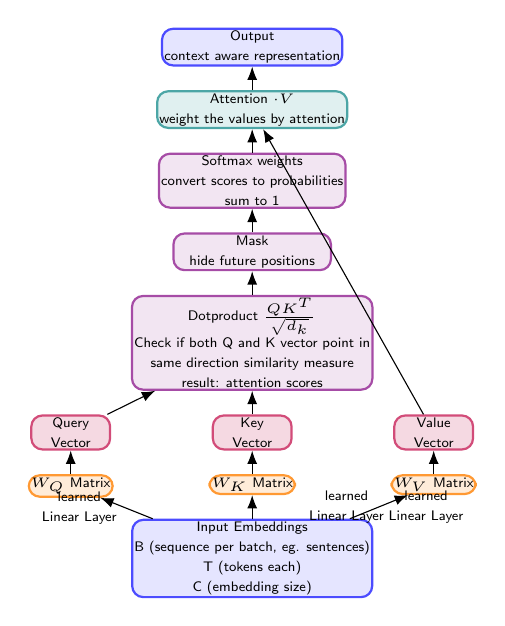
\begin{tikzpicture}[
  node distance=3mm and 2mm,  % <<< CHANGED: horizontal spacing smaller
  >=Latex,
  font=\tiny,
  block/.style={
    rectangle, rounded corners,
    draw, thick, align=center,
    inner sep=0.8pt,           % <<< CHANGED: slightly less padding
    minimum width=2cm,
  },
  input/.style={block, fill=blue!10, draw=blue!70},
  proj/.style={block, fill=orange!15, draw=orange!80, minimum width=1cm},
  vec/.style={block, fill=purple!15, draw=purple!70, minimum width=1cm},
  mid/.style={block, fill=violet!10, draw=violet!70},
  att/.style={block, fill=teal!12, draw=teal!70},
]

% --- Output ---
\node[input] (OUT) {Output\\ context aware representation};

% --- Weighted sum ---
\node[att, below=of OUT] (AV) {Attention $\cdot V$\\ weight the values by attention};

% --- Softmax / Mask / Score ---
\node[mid, below=of AV] (SM) {Softmax weights\\ convert scores to probabilities\\ sum to 1};
\node[mid, below=of SM] (MASK) {Mask\\ hide future positions};
\node[mid, below=of MASK] (SCORE) {Dotproduct $\frac{QK^T}{\sqrt{d_k}}$\\ Check if both Q and K vector point in \\same direction similarity measure\\result: attention scores};

% --- Q / K / V ---
\node[vec, below left=of SCORE, xshift=-0.5mm] (Q) {Query\\ Vector};   % <<< CHANGED
\node[vec, below=of SCORE] (K) {Key\\ Vector};
\node[vec, below right=of SCORE, xshift=0.5mm] (V) {Value\\ Vector};  % <<< CHANGED

% --- Projection matrices ---
\node[proj, below=of Q] (WQ) {$W_Q$ Matrix};
\node[proj, below=of K] (WK) {$W_K$ Matrix};
\node[proj, below=of V] (WV) {$W_V$ Matrix};

% --- Input ---
\node[input, below=of WK] (IN) {Input Embeddings\\
B (sequence per batch, eg. sentences)\\
T (tokens each)\\
C (embedding size)};

% --- Arrows ---
\draw[->] (IN) -- node[left, align=center] {learned\\ Linear Layer} (WQ);
\draw[->] (IN) -- node[right, align=center] {learned\\ Linear Layer} (WV);
\draw[->] (IN) -- node[midway, right, align=center, xshift=6mm] {learned\\ Linear Layer} (WK);

\draw[->] (WQ) -- (Q);
\draw[->] (WK) -- (K);
\draw[->] (WV) -- (V);

\draw[->] (Q) -- (SCORE);
\draw[->] (K) -- (SCORE);

\draw[->] (SCORE) -- (MASK);
\draw[->] (MASK) -- (SM);

\draw[->] (SM) -- (AV);
\draw[->] (V) -- (AV);

\draw[->] (AV) -- (OUT);

\end{tikzpicture}


{\footnotesize{Multi Head Attention}}

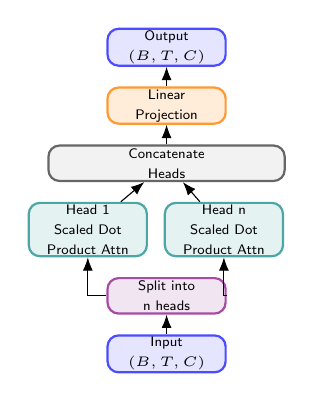
\begin{tikzpicture}[
  node distance=2.5mm and 3.5mm,   % <<< tighter overall
  >=Latex,
  font=\tiny,
  block/.style={
    rectangle, rounded corners,
    draw, thick, align=center,
    inner sep=0.7pt,
    minimum height=4.5mm,
    minimum width=1.5cm
  },
  wide/.style={
    block,
    minimum width=3.0cm
  },
  input/.style={block, fill=blue!10, draw=blue!70},
  mid/.style={block, fill=violet!10, draw=violet!70},
  head/.style={block, fill=teal!10, draw=teal!70},
  concat/.style={wide, fill=gray!10, draw=black!60},
  proj/.style={block, fill=orange!15, draw=orange!80},
]

% --- Top / output ---
\node[input] (OUT) {Output\\ $(B,T,C)$};

% --- Final projection + concat ---
\node[proj, below=of OUT] (WO) {Linear\\ Projection};
\node[concat, below=of WO] (CAT) {Concatenate\\ Heads};

% --- Heads: explicitly placed close together ---
\node[head, below=of CAT, xshift=-1cm] (H1) {Head 1\\ Scaled Dot\\ Product Attn};
\node[head, right=2mm of H1] (H2) {Head n\\ Scaled Dot\\ Product Attn};

% --- Split + input ---
\node[mid, below=of H1, xshift=1cm] (SPLIT) {Split into\\ n heads};
\node[input, below=of SPLIT] (IN) {Input\\ $(B,T,C)$};

% --- Arrows (BT) ---
\draw[->] (IN) -- (SPLIT);

\draw[->] (SPLIT) -| (H1);
\draw[->] (SPLIT) -| (H2);

\draw[->] (H1) -- (CAT);
\draw[->] (H2) -- (CAT);

\draw[->] (CAT) -- (WO);
\draw[->] (WO) -- (OUT);

\end{tikzpicture}

{\footnotesize{Transformers}}

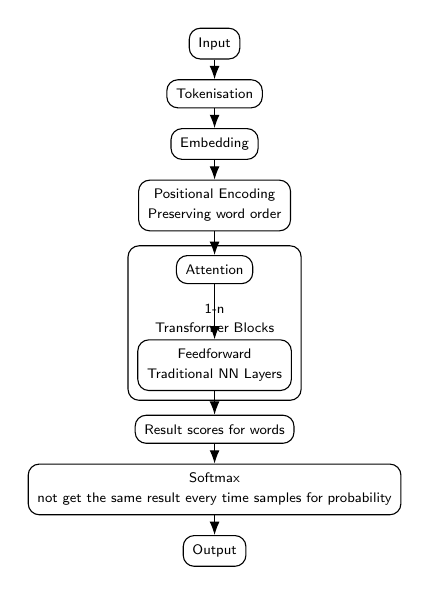
\begin{tikzpicture}[
  node distance=2.5mm and 3.5mm,   % <<< tighter overall
  >=Latex,
  font=\tiny,
  box/.style={draw, rounded corners, align=center},
  innerbox/.style={draw, rounded corners, align=center},
  bigbox/.style={draw, rounded corners},
  arrow/.style={-Latex, thick}
]

% Main vertical boxes
\node[box] (in) {Input};
\node[box, below=of in] (tok) {Tokenisation};
\node[box, below=of tok] (emb) {Embedding};
\node[box, below=of emb] (pos) {Positional Encoding \\Preserving word order};

% Transformer block (big box containing two inner boxes)
\node[innerbox, below=3mm of pos] (attn) {Attention};
\node[innerbox, below=7mm of attn] (ffn) {Feedforward\\Traditional NN Layers};

\node[bigbox, fit=(attn)(ffn)] (block) {1-n \\Transformer Blocks};

% Continue pipeline
\node[box, below=3mm of ffn] (res) {Result scores for words};
\node[box, below=of res] (softmax) {Softmax\\not get the same result every time samples for probability};
\node[box, below=of softmax] (out) {Output};

% Arrows
\draw[->] (in) -- (tok);
\draw[->] (tok) -- (emb);
\draw[->] (emb) -- (pos);
\draw[->] (pos) -- (attn);
\draw[->] (attn) -- (ffn);
\draw[->] (ffn) -- (res);
\draw[->] (res) -- (softmax);
\draw[->] (softmax) -- (out);

\end{tikzpicture}

    
\end{multicols}

\textcolor{red}{Sample Exam Questions}

Explain the progression from Bag-of-Words to learned embeddings:
a) What are the key limitations of binary Bag-of-Words representations? (List at least 3)
b) How do learned embeddings address these limitations?
A student says: "Why do we need attention? RNNs already have memory through their hidden state."
a) Explain the fundamental bottleneck problem with RNNs when processing long sequences.
b) Draw a simple diagram showing how information flows in:
– An RNN processing a 10-word sentence
– A transformer with attention processing the same sentence


1. Was ist zu beachten beim Implementieren von einem LLM-Agent? 
2. was sind die Unterschiede zwischen 1-hot Vektoren (tf-idf) und dichte Vektore (word2vec) 
3. was sind die Unterschiede zwischen word2vec und BERT? 


\end{landscape}
\end{document}